% ======================================================================
\section{Complexity}\label{sec:complexity}
Let the leaves have $n_0$ rows and $p_0$ columns, and let all ranks be at most $r$. One leaf costs
$O(p_0(n_0+r)^2)$: the QR factorization of the $p_0\times(\ell+n_0)$ matrix $[V_\tau,\,D_\tau^*]$ in the
size reduction dominates, and the QL factorization, the products with $P_\tau$ and $Q_\tau$ and the
triangular solve are of the same or lower order. There are about $m/n_0$ leaves. Every reduced node has
at most $2r$ rows and $4r$ columns, so it costs $O(r^3)$, and there are fewer than $m/n_0$ of them.
The right-hand-side update~\eqref{eq:bbar} is one HSS product per level, $O(m(n_0+r))$ at the leaf level
and less above. With $mp_0/n_0=n$,
\[
\text{time}=O\!\Big(n\,(n_0+r)^2+\tfrac{m}{n_0}\,r^3\Big)=O(n\,r^2)\quad\text{for }n_0\sim r,
\qquad \text{memory}=O(n(n_0+r)).
\]
At a fixed leaf size the cost is linear in $n$. Once the factors are computed, a solve with a new
right-hand side costs $O(n(n_0+r))$, i.e.\ $O(nr)$ for $n_0\sim r$: triangular solves, small unitary
products and one HSS product per level. By comparison, the dense minimum-norm solve costs $O(m^2n)$,
and conjugate gradients on $HH^*$ (CGNE) costs two HSS products per iteration with an iteration count
that grows with $\kappa(H)$.

Figure~\ref{fig:complexity} shows measured times for random HSS matrices with $m=n/2$ (family F2 of
Section~\ref{subsec:testmatrices}) and for families F1--F5, up to $n=\EfourMaxN$, with leaves of 200--400
rows. The time of the first solve, which computes the factors, grows linearly
in $n$ for every family (fitted exponents $\EfourSlopeMin$--$\EfourSlopeMax$ over the last four sizes), and so
does the time of a repeat solve with the stored factors (exponents
$\EfourSlopeRepeatMin$--$\EfourSlopeRepeatMax$). At the largest size a repeat solve is \EfourRatioRepeat{}
times faster than the first solve and costs as much as \EfourRepeatMatvec{} HSS matrix--vector products.
The dense QR solve grows like $n^{\EfourDenseSlope}$ and is $\EfourDenseRatio\times$ slower than the first ULV
solve at $n=\EfourDenseN$. CGNE needs \EfourCgIts{} iterations even on these well-conditioned matrices, each
with two HSS products; at $n=\EfourCgN$ it is $\EfourCgRatio\times$ slower than the first ULV solve and
$\EfourCgRatioRepeat\times$ slower than a repeat solve, and Section~\ref{subsec:stab} shows that it stops
converging as $\kappa$ grows. The timings come from
\texttt{mp\_exp\_scaling.m}.

\begin{figure}[!htb]
\centering
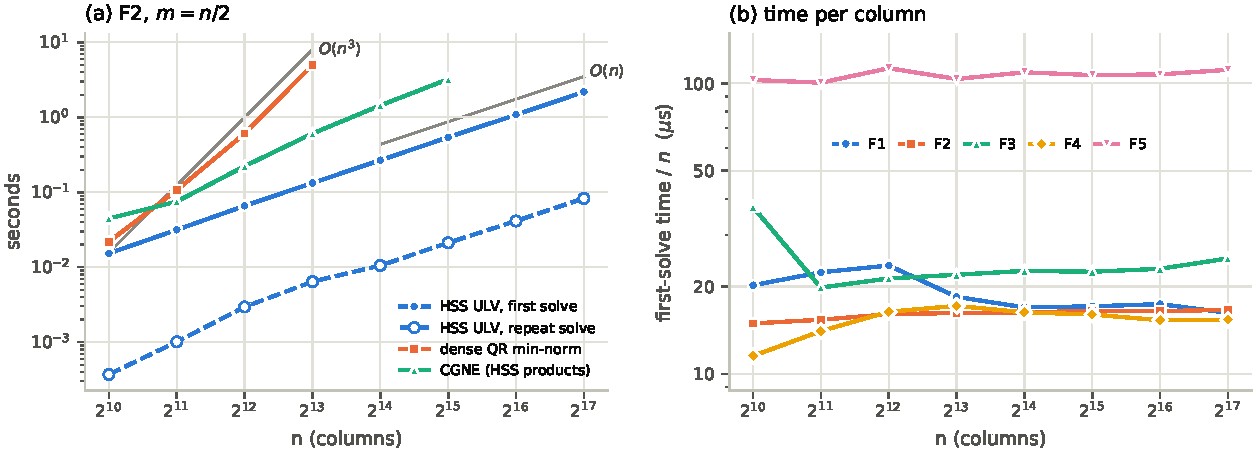
\includegraphics[width=\textwidth]{figures/m1_complexity.pdf}
\caption{Measured cost. (a) F2, $m=n/2$, rank 10: first solve (factorization and solve), repeat solve
with the stored factors, dense QR minimum-norm solve and CGNE (conjugate gradients on $HH^*$ with HSS
products, to relative residual $10^{-12}$); grey lines $O(n)$ and $O(n^3)$. (b) Time of the first solve
divided by $n$, for F1--F5: a flat line is linear cost (the first F3 point is a single dense block).
Times from \TimingPlatform; HSS solves are the median of three runs after a warm-up, each first solve
starting without stored factors; dense QR and CGNE are single runs.}
\label{fig:complexity}
\end{figure}
